% arara: xelatex
% arara: xelatex
% arara: xelatex


% options:
% thesis=B bachelor's thesis
% thesis=M master's thesis
% czech thesis in Czech language
% english thesis in English language
% hidelinks remove colour boxes around hyperlinks

\documentclass[thesis=B,english]{FITthesis}[2019/12/23]

%\usepackage[utf8]{inputenc} % LaTeX source encoded as UTF-8
% \usepackage[latin2]{inputenc} % LaTeX source encoded as ISO-8859-2
% \usepackage[cp1250]{inputenc} % LaTeX source encoded as Windows-1250

% \usepackage{subfig} %subfigures
% \usepackage{amsmath} %advanced maths
% \usepackage{amssymb} %additional math symbols

\usepackage{dirtree} %directory tree visualisation
\usepackage{graphicx}
\usepackage{tocbibind}
\usepackage[T1]{fontenc}
\usepackage{float}
\graphicspath{ {./images/} }

% % list of acronyms
% \usepackage[acronym,nonumberlist,toc,numberedsection=autolabel]{glossaries}
% \iflanguage{czech}{\renewcommand*{\acronymname}{Seznam pou{\v z}it{\' y}ch zkratek}}{}
% \makeglossaries

% % % % % % % % % % % % % % % % % % % % % % % % % % % % % % 
% EDIT THIS
% % % % % % % % % % % % % % % % % % % % % % % % % % % % % % 

\department{Department of Software Engineering}
\title{Cluster infrastructure for LearnShell}
\authorGN{Samuel} %author's given name/names
\authorFN{Majoroš} %author's surname
\author{Samuel Majoroš} %author's name without academic degrees
\authorWithDegrees{Samuel Majoroš} %author's name with academic degrees
\supervisor{Jakub Žitný}
\abstractEN{The main goal of this thesis is to present a functional cluster infrastructure for the LearnShell 2.0 project used by the Czech Technical University in Prague. To achieve this, we shall describe the current infrastructure and scrutinize today's pre-eminent technologies for container orchestration. Then, we shall present a basic cluster on which the LearnShell project is to be hosted, and define CI/CD routines for the services contained therein by utilizing Gitlab CI. We will document our code thoroughly and display our code in a separate repository.}
\abstractCS{Hlavným cieľom tejto práce je uvedenie funkčnej klastrovej infraštruktúry pre projekt LearnShell 2.0, ktorý je používaný Českou Technickou Univerzitou v Prahe. Aby sme dosiahli tento cieľ, najprv opíšeme súčasnú infraštruktúru a posúdime dnešné najznámejšie technológie pre kontajnerovú orchestráciu. Následne predstavíme jednoduchý klaster, na ktorom bude LearnShell hostovaný, a zadefinujeme CI/CD rutiny pre v klastri existujúce servisy. Budeme náš kód pozorne zdokumentuvávať a kód predvedieme vo svojom vlastnom repozitári.}
\placeForDeclarationOfAuthenticity{Prague}
\keywordsCS{Kubernetes, Helm, Docker, Docker Swarm, Gitlab CI, Google Cloud, Linux, LearnShell}
\keywordsEN{Kubernetes, Helm, Docker, Docker Swarm, Gitlab CI, Google Cloud, Linux, LearnShell}
\declarationOfAuthenticityOption{1} %select as appropriate, according to the desired license (integer 1-6)
% \website{http://site.example/thesis} %optional thesis URL


\begin{document}

% \newacronym{CVUT}{{\v C}VUT}{{\v C}esk{\' e} vysok{\' e} u{\v c}en{\' i} technick{\' e} v Praze}
% \newacronym{FIT}{FIT}{Fakulta informa{\v c}n{\' i}ch technologi{\' i}}

\setsecnumdepth{part}
\chapter{Introduction}

As we become ever reliant on internet-based technology in our daily lives, it stands to reason that there is a pervasive demand on software that is safe, accessible, and most importantly, dependable. More and more, we are growing accustomed to using the internet for even the most trivial of things, such as ordering food, or looking up the correct spelling of certain words. Therefore, web applications are ever increasingly throttled by an uncountable amount of requests from users, and it is of great importance that technology adapts to this challenge by employing new methods of creating an infrastructure that is scalable in a way that makes it impossible to be overwhelmed by too many requests to the point of system failure. In this thesis, we shall attempt to explain the theory behind, as well as the need for, containerization and orchestration as catch-all solutions to many problems troubling today's web applications. More specifically, we shall try and implement a basic cluster, on which the LearnShell portal of the Czech Technical University in Prague could run in the near future. 
\newline
In summary, these will be the main goals of the thesis:
\begin{itemize}
  \setlength\itemsep{0em}
  \item Analyze the current infrastructure architecture of LearnShell
  \item Explain the virtues of containerization and orchestration, as well as their history
  \item Compare existing orchestration technologies used in practice as well as their suitability for orchestrating LearnShell containers
  \item Implement a basic cluster, based on cutting edge orchestration systems
  \item Explore implementation of continous integration in LearnShell, specifically the newly created cluster
\end{itemize}


\setsecnumdepth{all}
\chapter{Architecture of LearnShell}

In this chapter, we shall take a closer look at the architecture of LearnShell. 
\newline
\newline
Before that, let us briefly describe its history. The first version of LearnShell was designed and built by Karel Jilek, a student of the Czech Technical University in Prague. In his bachelor's thesis, titled "Command and script testing system for bash language", he explains that the goal of this system would be to create an environment that would be able to verify the validity of a bash script by simply comparing the output of that script with the output provided by the system. \cite{learnshell-jilek} Later on, LearnShell would be used in the course "Programming in Shell 1" to evaluate assignments and exams specific to Bash programming. Eventually, a newer version, called "LearnShell 2.0" was introduced. This version would build upon the old one, providing new features, such as a plagiarism detection system, a logging system, as well as introducing a newer front-end design. And last but not least, a cluster would be created on which the application was to be deployed. In this chapter (and by extension this thesis), we shall focus on describing the state of affairs in the 2.0 version, as this is the version on which work is being done at the moment.
\newline
\newline
Now, let us begin with an overview of the architecture. Next, we shall focus on each separate piece of the puzzle as well as the tech stack in use.

\section{Overview}

The current production-ready version of LearnShell is composed of six containers that are connected each other on their local network, alongside an evaluator service that runs on its own server. Each of those services fulfill a specific role, as we will elaborate in the following subsections. In practice, the term for this is "microservice architecture", which can be succintly described as a collection of small, autonomous services that work together. \cite{building-microservices} 
\newline
In general, such an architecture adheres to principles of deployability and modifiability. \cite{building-microservices,architecting-chen} Meaning that by compartmentalizing your application into several smaller pieces, one can easily modify and later, deploy one part of the entire application without having to include the other parts, therefore avoiding issues such as having to compile the entire application after changing just one small piece of it. It is therefore only logical that in the case of LearnShell, lightweight, easily configurable containers, in the form of Docker containers, are used to divide the application into smaller parts, or packages. Not only that, but these containers are fairly simple to get running via configuration files. These containers communicate with each others via HTTP requests that work like glue holding the entire application together. \cite{microservices}
\newline
In the case of LearnShell, six containers in total are used as of right now. In the following sections, we shall briefly explain the functionality of each containerised package (plus the evaluator) in concise terms, as well as the technologies used by those packages. However, to get a full understanding of the inner workings of the application, it is advised to read the bachelor's thesis of Karel Jilek on this subject.
\newline
As a side note, even though the current architecture of LearnShell leans towards a microservices-based one, it is definitely not an example of an application purely made of microservices; for example, the backend service combines several features, such as an administration panel and a GraphQL together, and as such doesn't fit the bill of a microservice and is closer to a monolithic application in it scope. Nonetheless, the generator and evaluator only fulfill one specific role each, and are therefore much closer to the definition of a microservice. Since LearnShell is production-ready software, it is quite natural that it doesn't perfectly adhere to one paradigm, as that is nigh-on-impossible to achieve in practice.

\section{Architecture}

\subsection{Proxy server}

For the purpose of receiving incoming traffic and redirecting it, a container is used as a proxy server, which redirects requests received from the client, and points them toward containers for further processing, and sending back responses to the client received from these same containers as if it was by itself their origin, therefore fulfilling the role of a reverse proxy. \cite{proxies} A subdomain of the fit.cvut.cz domain is assigned to the ip address of this proxy server.
\newline
For all this, nginx was chosen as the most suitable candidate. As of 2021, Nginx is the most commonly used web server, and is renowned for its performance and ease of use. \cite{netcraft} Naturally, a well-maintained Docker image is available publicly on DockerHub, and there is no reason not to use it in production in this application, as well.

\subsection{Front end}

This container contains the code for the front end side of the application. As well as responding with the HTTP response, including assets such as CSS files and images to display on the client side, it also sends GraphQL queries to other containers, for example to create or display assignments. 
\newline
It is built entirely with Next.js, a modern JavaScript framework based on React, improving on it by adding most importantly a built-in routing system (by default, React does not contain one, and additional libraries, such as React Router, must be used) and several additional features such as server-side rendering or faster page loading by virtue of automatic code splitting.

\subsection{Back end}

The code in this container represents the data access layer of the application. Among its functionalities is writing and reading data to the database (such as users and assignments) and communicating with the generator and evaluator services for the purpose of creating randomized data for validation of Bash scripts and evaluating the outputs of these scripts by comparing them with the generated data. \cite{learnshell-borsky} The back end also communicates with KOS, our student information system, and an integration with the system for grades and evaluations, Grades, is planned for the future.
\newline
The entire back end is built in Django, a MVP (stands for model view presenter) web framework written in Python. In addition, the container contains several Bash scripts to ensure, among other things, connection and migration of data to the database, as well as configuration files for the web server.

\subsection{Distributed task queue}

In order to enable LearnShell to parallelize tasks related to generation of inputs and evaluation of Bash scripts, a distributed task queue is used. This comes in handy because not all of those tasks are completed in the same time horizon; therefore by using the distributed tasks queue, long running tasks are "worked on" by the services to which these tasks are assigned, namely generator or evaluator, while simple tasks such as data retrieval are still executed without having to wait for long running tasks to finish.
\newline
The technologies used here are the Python library Celery, which provides with all the tools required to for the purposes of running a queue on LearnShell, while we use a key-value database, Redis as an in-memory database on which the information regarding jobs is stored in a queue until these jobs are finished. Both the generator and the evaluator use their own distributed task queue, with generator using a containerised one and the evaluator running on its own server for now.

\subsection{Database}

Alongside Redis, the only stateful service in the application, a SQL database is used to store all important data persistently. The database contains information regarding users and their privileges, all the jobs performed by celery, assignments and exams created by teachers and submissions by students. LearnShell utilizes the PostgreSQL engine, although there is no particular reason to use it; it boiled down to the initial author's preference.

\subsection{Generator}

To elaborate on what was already mentioned in the back end subsection, the function of the generator service is the generation of randomized data for validation of LearnShell assignments and exams. 

Solely for this reason, the LearnShell Input-Describing Language (LI-DL for short) was developed, a sort of minimalistic domain specific language with a syntax similar to JSON that generates custom assignments as well as test cases, which the evaluator compares with the output of a shell script that is turned in by the user. \cite{learnshell-jilek}  
 
\subsection{Evaluator}

The evaluator, as befits its name, fulfills the role of a service that assesses each submission made by the user. It does so by creating a chroot jail, which is essentially a simulated root environment running on a directory; this way, the directory in question is isolated from the rest of the computer, protecting the computer from potential destructive effects of certain commands, such as the famous fork bomb. \cite{unix-handbook} It checks for criteria such as whether the user created or deleted the correct files, whether the files created have the correct permissions, or the outputs (and the streams through which they are passed) of the scripts submitted.
\newline
Currently, the evaluator runs on its own server, and therefore is the only service which is not packaged inside of a container.

\section{Potential improvements}

Even though the application does all that it sets out to do, there are always areas of improvement, which we shall point out in the following subsections.

\subsection{Evaluator containerization}

\subsection{Functionality-related improvements}

\subsection{Cluster}


\chapter{Containerization and Orchestration}

In this chapter, we shall finally explain in detail the terms containerization and orchestration; they are of such importance to this thesis that a separate chapter is necessary to elaborate on the theoretical concepts as well as their practical applications. Finally, we will review the most used solutions for container orchestration, and in the next chapter, we are going to compare their use cases in general and specifically to LearnShell. Take note that there is a section specially dedicated to Kubernetes because of its complexity as well as its particular merit within our application.

\section{Theoretical concepts}

\subsection{Virtualization}

In days of yore, the only viable way for most companies to work out an IT infrastructure and provision servers for a company was by spending considerable resources on buying physical servers, that is, by spending money on computers and computer parts and running the servers on them. Although it works at first glance, there is an issue which becomes apparent at scale; mismanagement of the machine’s resources, be it its RAM, CPU, or physical memory. In simple terms, two problems could arise; either the company would underspend, and buy less physical machines than was necessary, which would lead to recurring outages and stress before new servers could be provisioned to support the ever increasing amount of users. Another potential disaster could be caused by the company overspending and sinking way more resources into buying and provisioning servers before it was necessary, therefore wasting money that could be used for different purposes.
\newline
Ideas of creating some sort of abstraction appeared in the 60’s, when Jim Rymarczyk from IBM worked out a way to host multiple operating systems on the same piece of hardware, using a hypervisor, which is a software, firmware or hardware that creates virtual machines, emulations of computer systems running their own operating systems. This type of hypervisor would stand directly above the hardware in hierarchy, and host multiple virtual machines on top of it. \cite{virtualization}
\newline
Later on, at the tail end of the century, a newer virtualization model to provide abstraction of virtualized resources was developed by the engineers at VMWare. \cite{vmware} It would employ a hosted hypervisor, which means that the hypervisor would be run on a host operating system, making it much easier to manage virtual machines, therefore making virtualization more viable than ever before. \cite{virtualization}
\newline
However, VM-based virtualization still effectively “carves out” a part of the hardware resources of the physical server, as it creates a full-fledged operating system which treats its allocated hardware as if it was the only operating system running on it.
\newline
With the advent of Docker, container-based virtualization (henceforth referred to as containerization) turned into an extremely popular virtualization technique, which we shall describe in the following chapter. 


\subsection{Containerization}

Even though containerization has been around for decades before Docker, for example in the form of BSD “jails”, it is only with the creation of Docker that it truly hit its stride. As seen on the diagrams, the difference between VM-based and container-based virtualization lies mainly in the fact that while VM-based virtualization creates (virtualizes) an entire operating system, with abstractions for hardware such as virtual CPUs and virtual disks, container-based virtualization uses techniques within the kernel to only virtualize the non-hardware aspects of the operating system, creating a separate root filesystem or network system, while not emulating hardware at all.
\newline
This opens up a whole new world of possibilities. Thanks to the efficiency and fast start-up caused by using far fewer resources than full-fledged virtual machines, as well as the opportunity to create truly specialized containers that only focus on providing one service without any redundancies, it’s now possible to manage these containers in such a way that it’s much easier to integrate these services together in a container-based architecture with the added benefit of greater security and easier scaling if each container only has one job.
\newline
These containers can then be efficiently managed, upgraded and be overseen by tools built specifically for the configuration and management of containers, also known as container-orchestration systems, with the most commonly used at the moment being Kubernetes, or K8s for short.


\subsection{Orchestration}

As we move into a container-based architecture, in which several microservices delegate tasks and communicate with each other, there arises a need to manage the containers, their lifecycles and the relations between them. This is where the term container orchestration comes in.
\newline
There are several tasks which are managed by orchestration tools, such as the provisioning and deployment of containers, health checks of these containers, managing the allocation of resources between these containers and many more. 
\newline
More broadly, orchestration is the automated configuration and coordination of systems and software in general. However, in this particular thesis, we shall focus on container orchestration in particular, that is, on the management of containers.
\newline
At this moment in time, the most popular container orchestration software by far is Kubernetes, as mentioned in the previous section, however, Docker Swarm is another such tool that posits itself as easier to use, and therefore preferable in certain cases. We shall describe these two platforms and the differences between them in more detail in some of the next sections, as well as a chapter dedicated to Kubernetes.


\subsection{Cloud computing}

Even though the umbrella term "cloud computing" is not directly connected to orchestration, it might be worth it to give an overview here, as there are numerous immediate and powerful benefits of running clusters on the cloud.
\newline
As defined by one of the foremost cloud computing corporations in the world, the cloud can simply be described as a collection of servers located all over the world that can be accessed over the Internet, as well as the software and databases that run on those servers. Therefore, by accessing the cloud, users and companies don't need to manage physical servers or run software applications on their own machines. \cite{cloudflare} The rise of cloud computing was revolutionary, as it led to widespread adoption over the years by companies small and large, not at all limited to technology. The staggering upwards trend in the revenue of the cloud computing market over the last few years should serve as sufficient proof. In fact, since 2016, the total cloud market revenue has tripled in value, from around eight billion dollars to little more than twenty-four. \cite{cloud-market}
\newline
In practice, the adoption of cloud computing by companies (or communities) enables the developers to stop worrying about earthly matters like the state of their physical machines, on which the application is running, and allows them to delegate it entirely to the cloud provider. The business model works on a pay-as-you-go approach for every cloud provider that is relevant in today's market, meaning that the customers periodically receive a bill based on criteria such as how much data is stored on the cloud, or how many instances of virtual machines are currently running. \cite{aws-framework} An early adopter, Amazon set the trend with Amazon Web Services in 2006, with Microsoft (Azure) and Google (Google Cloud) following suit. Up to this day, Amazon retains a mamooth share of the total cloud computing market revenue, as well as a huge amount of diverse services, with Microsoft catching up and Google having found its niche in Kubernetes offerings. Currently, all cloud providers are making leaps and strides in maintaining and updating services built specifically for enabling the users to create Kubernetes clusters on the cloud, with Google generally being considered as the best choice, by virtue of it being the main driving force behind the existence of Kubernetes itself.
\newline
As for this thesis, a testing cluster was built using Google Cloud and its Google Kubernetes Engine, demonstrating the power of cloud computing in practice. More on this will be revealed in the last chapter.


\section{Containerization technologies}

After explaining some of the theory, let's take a look at some of the most used, tried and tested containerization and orchestration software nowadays. All of the following tools play a huge role in today's tech world, and it could be said that the advent of microservice-based architecture is largely thanks to these tools. In addition, we will demonstrate a real-world application of these tools in the last chapter, showcasing the Kubernetes cluster made for LearnShell.

\subsection{Docker}

Today, Docker is without any doubt the pre-eminent software for containerization. It was originally meant to be merely an internal PaaS (Platform as a Service) tool for dotCloud, an European company, however, it quickly gained traction as many truly big companies, for example Microsoft and Google, started noticing the numerous tangible benefits provided by switching to Docker in production. \cite{docker-java} This led to a huge amount of resources being spent on the development and improvement of the Docker project, with several off-shoot tools created as a result, such as Docker Compose, or Docker Swarm.
\newline
Even though Docker is a complex piece of software, using it in practice is not as difficult as one may think. Generally, it boils down to writing a configuration file called a Dockerfile. Within the Dockerfile, the user specifies several parameters, such as commands that are to be executed upon deployment of the container, and most importantly, using the FROM keyword, the base image from which the container is to be derived. This image will be downloaded from Dockerhub, which is essentially a public repository of pre-configured images, with minimal overhead. 
\newline
Generally, the most commonly used terms in the Docker world are “container” and the aforementioned “image”. An image is an immutable (read-only) file that contains the source code, dependancies and libraries from which the container is built. On the other hand, a container is a virtualized run-time environment which is created from the image which serves as a template. \cite{docker-phoenix} It is completely isolated from the system on which it runs as well as extremely lightweight in comparison to a virtual machine, mainly due to being virtualized on the application layer instead of the hardware layer of the machine. 
\newline
Docker images are stored in registries, which can be either public or private. By running a command inside of the shell, the user can specify an image name as well as a repository and a tag (signifying the version of the wanted image), in order to use that image as a template from which to create a local container. There are numerous repository offerings, that is platforms on which one may host a registry. The most popular by far is DockerHub, however for purposes such as cloud integration, paid registries can be maintained by cloud providers and other corporations, such as Amazon ECR, Google Cloud Container Registry or Gitlab Private Registry. Additionally, it is possible (and sometimes preferable) to host a local registry, although it requires additional setting up.

\subsection{Docker Compose}

Not long after its conception, Docker became ubiquitous in software engineering, as it enabled huge projects to be smoothly divided into containers, each doing its own part independent of the other, moving from a monolithic architecture to a microservices-based one. As projects increase in scope, the amount of containers naturally increases as well, and with it the complexity of running them and managing their interactions. For this reason, Docker Compose was developed to be a tool that enables the user to create and start multiple services within their respective containers. All this can be performed by specifying a YAML file, docker-compose.yaml, and running it from the command line to deploy a multi-container application. \cite{docker-compose-docs}
\newline
In addition, one can specify a bridge network on which the containers defined by Docker Compose may communicate.

\section{Orchestration technologies}

Now that we have exposed the seminal containerization technology in Docker, it is time to focus on the most used solutions for orchestration, starting with Docker Swarm.

\subsection{Docker Swarm}

Bridging the gap between containerization and orchestration, Docker Swarm is, alongside Kubernetes, as of today the most used tool for creating and managing a cluster. It was created as a lightweight, easy-to-use alternative for cluster provisioning, enabling the user to quickly get up to speed and set up a cluster, which is colloquially referred to as “swarm” in the Docker nomenclature. As we have ultimately decided to go for Kubernetes as our technology to create a LearnShell cluster, we shall give a concise description of Docker Swarm in this subsection, followed by a comparison with Kubernetes in the next section. However, we shall not delve deep into the details, as this would be beyond the scope of the thesis.
\newline
The architecture of a swarm consists of several Docker hosts, that is server (be it on virtual machines, or physical ones) on which an installation of the Docker engine is present, and one or more containers are running. \cite{swarm-key-concepts} Those are called nodes. There are two, and only two, types of nodes; the manager node and the worker node. The nomenclature is fairly self-explanatory. While the worker nodes only serve as vessels for containers contained therein, the manager nodes, in addition of possessing all the capabilities of worker nodes, also fulfill the function of maintaining the state of the swarm and the communication of its nodes, as well the scheduling of services. In a swarm, a service is a definition of tasks to be executed on a node. \cite{swarm-nodes} For example, one may define a service to be a container created from an image pulled from a registry, which is thereupon provided with a command that is to be executed once the container is up and running. Therefore, when running a swarm and aiming to run a container on a worker node, one should first create the node, and then define a service to run a container on that same node.
\newline
In order to allow each node to transfer data between them, a network can be established by using the overlay network driver as well as the bridge network driver. The overlay network driver, also called ingress, handles traffic to a swarm service from outside, while the bridge network driver connects the Docker daemon one host to another Docker daemon on another host. 

In a way, although take note that this is merely the personal opinion of the author, the terminology of Docker Swarm may differ from that of Kubernetes, yet there are often essentially addressing the same concepts. For example, a Node in Docker Swarm is very similar to a Pod in Kubernetes, a docker config is very similar to a ConfigMap, et cetera. Therefore, it appears that the two orchestration solutions are quite a bit closer in their execution than one might think at first glance.


\section{Kubernetes}

In this chapter, we will dive deep into the inner workings of Kubernetes, our orchestration platform of choice. For the reasons why we shall be using Kubernetes in our LearnShell cluster, see the next chapter, specifically the section "Docker Swarm vs Kubernetes".
\newline
To quote the official documentation; "Kubernetes, also known as K8s, is an open-source system for automating deployment, scaling, and management of containerized applications". \cite{kube-documentation}

\subsection{History}

Kubernetes was developed and launched by many of the same developers that used to work on Borg, Google's internal platform for cluster management. \cite{unix-handbook} These same developers would later work on Omega, which was to be the second generation of Borg, and still an internal, proprietary tool used by Google. Finally, in 2014, the Kubernetes project started in full swing, with the ambition to present an open-source, truly multi-purpose orchestration system, using both the experiences of Google's developers that worked on Borg and Omega years before as well as the power of the open-source community. \cite{medium-kube-history}
\newline
The very first version of Kubernetes was released to the public on July 21, 2015, and a partnership with the Cloud Native Computing Foundation was made, boosting development manpower significantly. Later on, in 2016, the first package manager for Kubernetes was released, called Helm, which we shall be using in our cluster, as it is a very powerful addition to the Kubernetes ecosystem. With each passing year, the adoption for Kubernetes is increasing, and this is reflected in the amount of commits on Github; based on new commits, its repository was the ninth most popular on Github in 2018. \cite{cncf-kube-graduate}

\subsection{Architecture}





\subsection{Building blocks}

\subsection{Pod}

\subsection{Deployment}

\subsection{Service}

\subsection{ConfigMap}

\subsection{Secret}

\subsection{Helm}

\subsection{Minikube}

\subsection{Cloud offerings}



\chapter{LearnShell Cluster Analysis}

In this chapter, which is the first of the two that describe the practical part of this thesis, we shall explain our architectual decisions as well as the motives behind them. We will describe the technologies used and why they were necessary, and where need be, we shall compare the most viable technologies for our particular use case.

\section{Docker Swarm vs. Kubernetes}

Since we will be implementing a cluster for LearnShell, one of the most important decisions we had to reach was to make an informed choice between Docker Swarm and Kubernetes as our orchestration platforms. Therefore, in this section, a comparison of Docker Swarm and Kubernetes will be made; for each platform, we shall describe the general use cases, the advantages and disadvantages, as well as their future in the industry. Then, we will concentrate on LearnShell specifically, and reach a final decision on which platform is the best for our use case in particular.

\subsection{General comparison}

As we have already discussed, the main practical difference between Docker Swarm and Kubernetes historically lied in their complexity. Docker Swarm is much more tied to Docker itself than Kubernetes, which supports several container runtimes. In fact, as of 2021, the default container runtime of the newest Kubernetes version is containerd. \cite{kube-containerd} In fact, swarm mode is natively included in Docker, so there's no need to install additional packages. As for Kubernetes, things aren't so simple, as we will elaborate later. 
\newline
Additionally, the learning curve is much steeper with Kubernetes, however, Kubernetes has a much, much more rich ecosystem, and as such there are many problems that can be easier to solve with Kubernetes than with Docker Swarm. Regardless of the learning curve of each platform, it has to be said that the documentation of both platforms is impeccably written, even though the author of this thesis finds that Kubernetes has an edge in this regard. One strength in particular is the option of running a test cluster via in-browser terminal, connecting to the cloud via SecureShell. This enables the user to immediately apply in practice what he has learned through reading the documentation. Therefore, it could be said in summary that while Docker Swarm is easier to grasp initially, both platforms have great documentation that explains the concepts quite capably, with Kubernetes being slightly better.
\newline
One area where Kubernetes has a clear, unassailable advantage is industry adoption. As proof, taking a look at the respective Github repositories of each platform should suffice (this is possible due to both platforms being open source from the very start, and as such all the code is publicly available). By glancing at the pull requests of each repository (in layman's terms, a pull request is a request for review of code before it is merged into a branch of a repository, and therefore integrated into the codebase), one can see that there is a world of difference; currently, the amount of pull requests for Kubernetes is ten times more than the amount for Docker Swarm. \cite{swarm-pull, kube-pull} Another important factor is that Kubernetes was initially developed, and is being maintained largely by Google; an industry behemoth. This means that there is a near-infinite reserve of resources dedicated to keeping Kubernetes alive and well.
\newline
Industry adoption spills over to many other factors, one of them being third-party support for a given orchestration platform. In this, Kubernetes is a clear winner. Each major cloud provider maintains a service designed specifically to simplify the creation of a cluster on the cloud, with Google Cloud naturally being the fan favorite, due to its close connection to the product. In addition to that, foremost git-repository managers provide an integration with Kubernetes, facilitating integration of the cluster into the DevOps lifecycle of the given project.
\newline
One notable factor that should not be underestimated, and is again tied to industry adoption, is the future of each platform. Kubernetes is currently extremely dominant in the orchestration space, and as such it is entirely possible that within the next few years, support for Docker Swarm could be dropped completely. The developer should take this into account, especially when it concerns any projects that should be here to stay, as migrating a large project from Docker Swarm to Kubernetes could be a challenging feat.
\newline
In summary; the strength of Docker Swarm lies in its shallow learning curve, as well as its seamless integration with other Docker offerings. However, Kubernetes wins in every other category; it is feature-rich, exquisitely documented and appears to be extremely dominant in comparison to Docker Swarm in the industry.

\subsection{Project-specific comparison}

Finally, it is time to take think about LearnShell specifically, and choose the best orchestration platform for our use case. We shall decide based on these criteria; ease of setting up a cluster, maintainability, versatility and integration with other services used by LearnShell.
\newline
When it comes to quickly setting up a cluster, Docker Swarm wins; its natural integration with other Docker services, such as Docker Compose, comes in really handy, as it allows us to run a few commands to get a cluster (or swarm, to adhere to the nomenclature) running. However, the rich ecosystem of Kubernetes holds its own here, as it gives us several options, such as Minikube or Kubernetes-in-Docker, to quickly set up a cluster. Nevertheless, a minimal understanding of how Kubernetes works is still necessary, and as such it remains true that a little more time reading the documentation will be necessary.
\newline
In the case of LearnShell, I define maintainability by the difficulty of keeping the cluster up and running, as well as updating the containers and adding new ones without disrupting it. Another important factor is how difficult it would be for new members of the LearnShell team to get up to speed with the cluster. In this case, the sheer size of the Kubernetes ecosystem plays a very important role, since any potential new developers have a plethora of articles, video, books or documentation on the internet at their disposal, while Docker Swarm is dwindling in its presence. Therefore, one can assume that if the cluster were to be improved upon in the future, it would be far easier to do so with Kubernetes, since it is certain to be a dominant player in the orchestration world for some time.
\newline
Versatility is admittedly a rather broad term to apply here, but in this case, we are addressing questions such as how difficult it would be for us to change up the proxy server on which LearnShell is running, or the database used by LearnShell, or (most importantly!) how easy or hard it would be to migrate the cluster from an on-premises architecture to the cloud. Whereas the services used by the cluster are quite easy to change up in both platforms, since Docker Swarm with its natural integration of Docker containers allows us to simply pull a different image if we wanted to use a different database engine, for example, and Helm makes this trivial with Kubernetes as well, it is the cloud where Kubernetes really shines here. Since there are comprehensive offerings on the cloud for Kubernetes, such as GKE on Google Cloud, it is entirely within the realms of possibility to migrate the entire cluster to the cloud. This could potentially not only lead to less upkeep, but to a much smoother experience of maintaining the cluster, especially now that GKE Autopilot was introduced, which promises greater optimization of resource use by the cluster, leading to greater performance in addition to lower costs of upkeep. \cite{autopilot}
\newline
The last criterion would be the integration with other services, which essentially points to future possibilities of running a continuous integration routine on Gitlab (where LearnShell repositories are hosted), in which it would be possible to automatically replace older versions of containers with new ones, or possibly keeping different clusters for different purposes, such as a staging cluster for testing purposes, and a production cluster, which the students and teachers would be using. In this, Kubernetes is a clear winner, as Gitlab is making a great effort in being containerization and orchestration friendly by allowing even free-tier users to integrate a cluster with their projects. \cite{gitlab-kube} Also, it coincidentally allows us to keep a private container registry for free, and creating CI routines with Gitlab Runners. However, unfortunately, for the purposes of LearnShell, there are only so many features that we can use at this moment in time, since the current release of Gitlab (11.8.0.) used by the university is more than two years old, and we are using the Community edition, which doesn't have some features that could prove very useful. Among these features is the Kubernetes Agent or Auto Devops, a platform that advertises reduced complexity in setting up pipelines, and probably most importantly in our case, the option to integrate multiple clusters into Gitlab, which would give us the option to have different pipelines, for example one for testing purposes, and one for the production cluster. Nevertheless, the option to use a private Gitlab registry remains available, as well as the option to use Gitlab Runners on our cluster to run CI pipelines; we shall elaborate on this later.
\newline
After much deliberation, we have decided to choose Kubernetes as our orchestration platform of choice. Even though the learning curve is undoubtedly quite a bit steeper than the alternative, what gives is its edge in the case of LearnShell is the fact that continous integration routines for the cluster are natively available within Gitlab, and that there is a strong argument for potentially migrating the cluster from on-premises to the cloud, as all the cloud providers are actively working on making this as painless as possible. Also, the industry adoption of Kubernetes leads to a great amount of resources being available in the case of troubleshooting the cluster.

\section{On-premises vs Cloud}

This section is dedicating to comparing the viability of hosting the LearnShell cluster on "bare metal" servers potentially provided by the university with hosting it entirely on the cloud, here represented specifically by GCP. As in the previous section, we shall first begin with a general comparison and then one dedicated to our project.

\subsection{General comparison}

While \cite{kube-on-prem}

\subsection{Project-specific comparison}

\subsection{Provider-independent solution}

There is one notable fact that should be called attention to; Kubernetes can be built rather easily to be as provider-independent as possible, and therefore it is viable to host a cluster on any cloud provider, as well as on-premises with minimal changes to the configuration files in which the cluster is to be defined. As such, our practical solution, which is in the following chapter, is made to be almost completely identical for both the on-premises cluster as well as for the GKE cluster with small differences here and there, which we shall take note of. With that in mind, we can easily move between an on-premises cluster and a cloud-hosted one, depending on the direction LearnShell goes in.

\section{Helm}



\section{Continuous integration and Continuous deployment}

\subsection{Gitlab CI}



\subsection{Private container registry}

In order for our cluster to run deployments, we need to provide Kubernetes with the necessary Docker images, from which to create containers contained within the pods maintained by these deployments. For that, there is a requirement for a container registry, wherein these images will be located. Also, for security reasons, this registry should be private; since LearnShell is currently only used by the Czech Technical University, its code should not be accessible from the outside, and therefore outsiders should not be able to pull LearnShell images without any authorization. From our research of possible private container registry offerings, we have arrived at a crossroads between three alternatives:

\begin{itemize}
  \setlength\itemsep{0em}
  \item Self-hosted registry
  \item Google Container Registry
  \item Gitlab Container Registry
\end{itemize}

Since we have deployed a cluster on Google Cloud, a natural option would be to also host our images there; it would enable for easy and robust integration with our GKE-hosted Kubernetes cluster. However, there is a monthly 
fee of 0.0026 dollars per GB per month, and we would like to avoid any monthly payments as much as possible. Therefore, we shall narrow our scope to free offerings. Out of those, we have only found two possibilities that are both free of charge as well as private. We could use a self-hosted registry, which is definitely possible. However, there are two disadvantages; since it is self-hosted, we would have to set it up, as well as maintain it manually, which could lead to trouble down the road, as we are trying to maximize automatization, and therefore avoid the need for manual maintenance. Secondly, such a solution would be harder to integrate with Gitlab and its CI \& CD offering; it would still be possible, but additional configuration would be necessary, increasing complexity. There is only one option that is both free, private and enables integration with Gitlab, and that is hosting the image registry on Gitlab itself, using the Gitlab Container Registry. This is also the best provider-independent option, as a DevOps pipeline on Gitlab would be easiest to improve upon by hosting the images there, as well.
\newline
As such, we arrive at the conclusion that Gitlab would be the ideal option for a private container registry.

\subsection{Gitlab Runners}

In order to facilitate effective CI \& CD for our LearnShell cluster, we should use as many boons as Gitlab can possibly provide. One of those would definitely be the Kubernetes group-level integration, which is provided in the Community edition. 





\chapter{LearnShell Cluster Implementation}

In this final chapter of our thesis, we shall focus completely on the practical side, which is the implementation of our cluster in practice. We shall provide an overview of our code, our directory structure as well as diagrams showing the cluster in its entirety. Also, we shall focus on some key decisions made during the process, potential alternatives, goals achieved, and finally, areas of improvement. However, be advised that we will not be going deep into theory, since that was already elaborated upon in the previous chapters.
\newline
Importantly, the cluster which we shall be focusing on in this chapter is the one running on Google Cloud, however, there is almost no difference between the on-premises cluster implementation and the cloud one; this is merely the personal preference of the author. Nevertheless, we shall call attention to any differences as we present our implementation.



\section{Technologies}

To start off, let us briefly summarize the main technologies we have made use of after our analysis:

\begin{itemize}
  \setlength\itemsep{0em}
  \item \textbf{Kubernetes} as our orchestration platform
  \item \textbf{Docker} as our containerisation platform
  \item \textbf{Gitlab Container Registry} as our private container registry
  \item \textbf{Helm} as our package manager
  \item \textbf{Google Cloud} as our cloud platform, and by extension \textbf{GKE} as our Kubernetes engine
  \item \textbf{Minikube} as our local development single-node cluster platform
  \item \textbf{Gitlab CI/CD} and \textbf{Gitlab Runners} to facilitate CI \& CD for LearnShell repositories
\end{itemize}

As a side note, we have used Linux as our operating system of choice both locally and on the cloud, due to its seamless integration with Docker. On Google Cloud, Linux we have deployed three VMs running Google's Container-optimized OS, which is tailor-made for running containers, as its name implies. These VMs were provisioned automatically by GKE in order to function as nodes (one control plane node, two worker nodes).
\newline
Less importantly, we have used Vim as our text editor due to its ease of use when editing configuration files and availability on machines on the cloud. 



\section{Project structure}

Let us continue with a brief overview of the project structure of the repository with our cluster configuration.

\begin{figure}[H]
\caption{Directory tree of the LearnShell Cluster project}
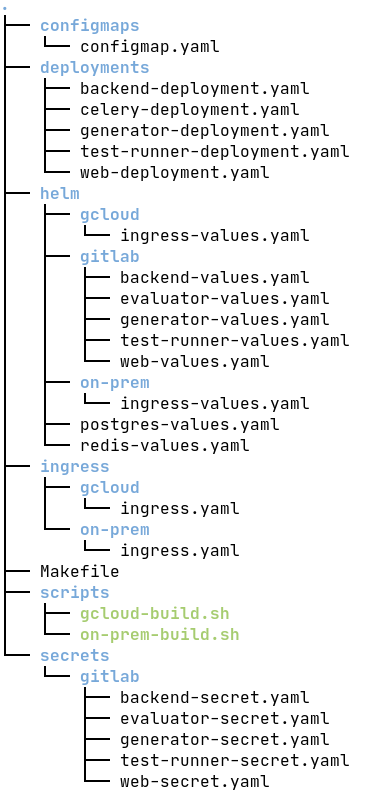
\includegraphics[scale=0.5]{tree-white-bg}
\end{figure}


As we can see from the output of running \verb|tree| in the project root, the files in our repository are almost exclusively either YAML configuration files or shell scripts, which is par for the course in a Kubernetes application; the YAML files contain instructions based on which we build all resources in our cluster, while the shell scripts use them to build our cluster from scratch.

Each directory in this project has its specific, fairly self-explanatory role. However, two directories deserve a little more in-depth explanation, and those are \verb|gcloud/| and \verb|on-prem/|. Those directories contain files specific for cluster implementations; if one were to run \verb|make gcloud|, for example, the script would ignore the contents of the \verb|on-prem| directories. In the end, we managed to keep the cluster configurations as provider-independent as possible, however, we could not avoid it in the case of Ingress, simply because gcloud only supports a version with a specific nomenclature (tagged as v1beta1). Nevertheless, once Google Cloud inevitably supports the newest version of Ingress, there will be no more need for separate implementations, so this is only a temporary measure.

\begin{figure}[H]
\caption{Line count of the LearnShell Cluster project}
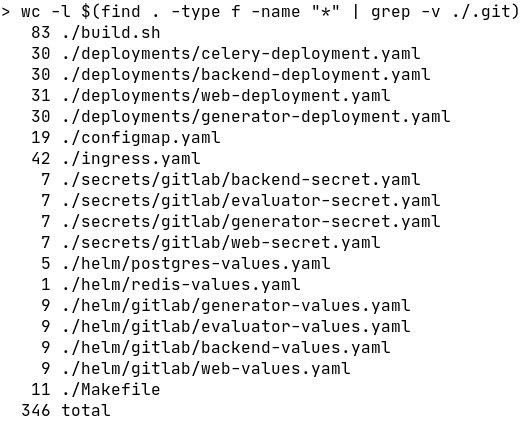
\includegraphics[scale=0.5]{line-count}
\end{figure}

By running \verb|wc -l| on all the (not auto-generated) files in the repository, we arrive at somewhere around 550 lines of code, with the bulk of it being in the deployment configurations and the shell scripts. With a little work, it would not be a problem to extend the project to include additional cloud provider options; the current set-up scripts are extremely similar, and can even be merged into one in the future, when cloud providers adopt the new standard of Ingress configuration.

\section{Functionality}

Before we get to any diagrams, we should properly explain what the project does. Essentially, it all boils down to our Makefile and shell scripts. By calling either \verb|make gcloud| or \verb|make on-prem|, a cluster is built from scratch in the default namespace, either on the GKE engine on Google Cloud, or locally on Minikube.

To further explain, creating these clusters via Makefile requires these prerequisites:

\begin{itemize}
  \setlength\itemsep{0em}
  \item \textbf{For both clusters}
  
  \begin{itemize}
    \setlength\itemsep{0em}
    \item Have the newest version of \textbf{Docker} and \textbf{Kubectl} installed on your machine.
    \item Use \textbf{Bash} as your shell in order to interpret the scripts.
  \end{itemize} 
  \item \textbf{For Google Cloud}
  
  \begin{itemize}
    \setlength\itemsep{0em}
    \item Run \verb|make gcloud| on a VM provisioned by GKE.
  \end{itemize}
  \item \textbf{For On-premises}
  
  \begin{itemize}
    \setlength\itemsep{0em}
    \item Have \textbf{Minikube} installed on your machine.
  \end{itemize}
\end{itemize}

Upon running the Makefile command, setting up the cluster could take several minutes; be advised that the process is far slower on the on-premises cluster, due to it running on Minikube, which is a single-node cluster. In comparison, the Google Cloud cluster uses GKE to make sure all the pre-provisioned nodes share the load of setting it up, and is therefore many times faster.

\section{Cluster}

In this section, we shall fully explore the cluster created by the project by utilizing diagrams and explanations. 

\subsection{Deployments}

\begin{figure}[H]
\centering
\caption{Deployments within our cluster}
\hspace*{-2cm}
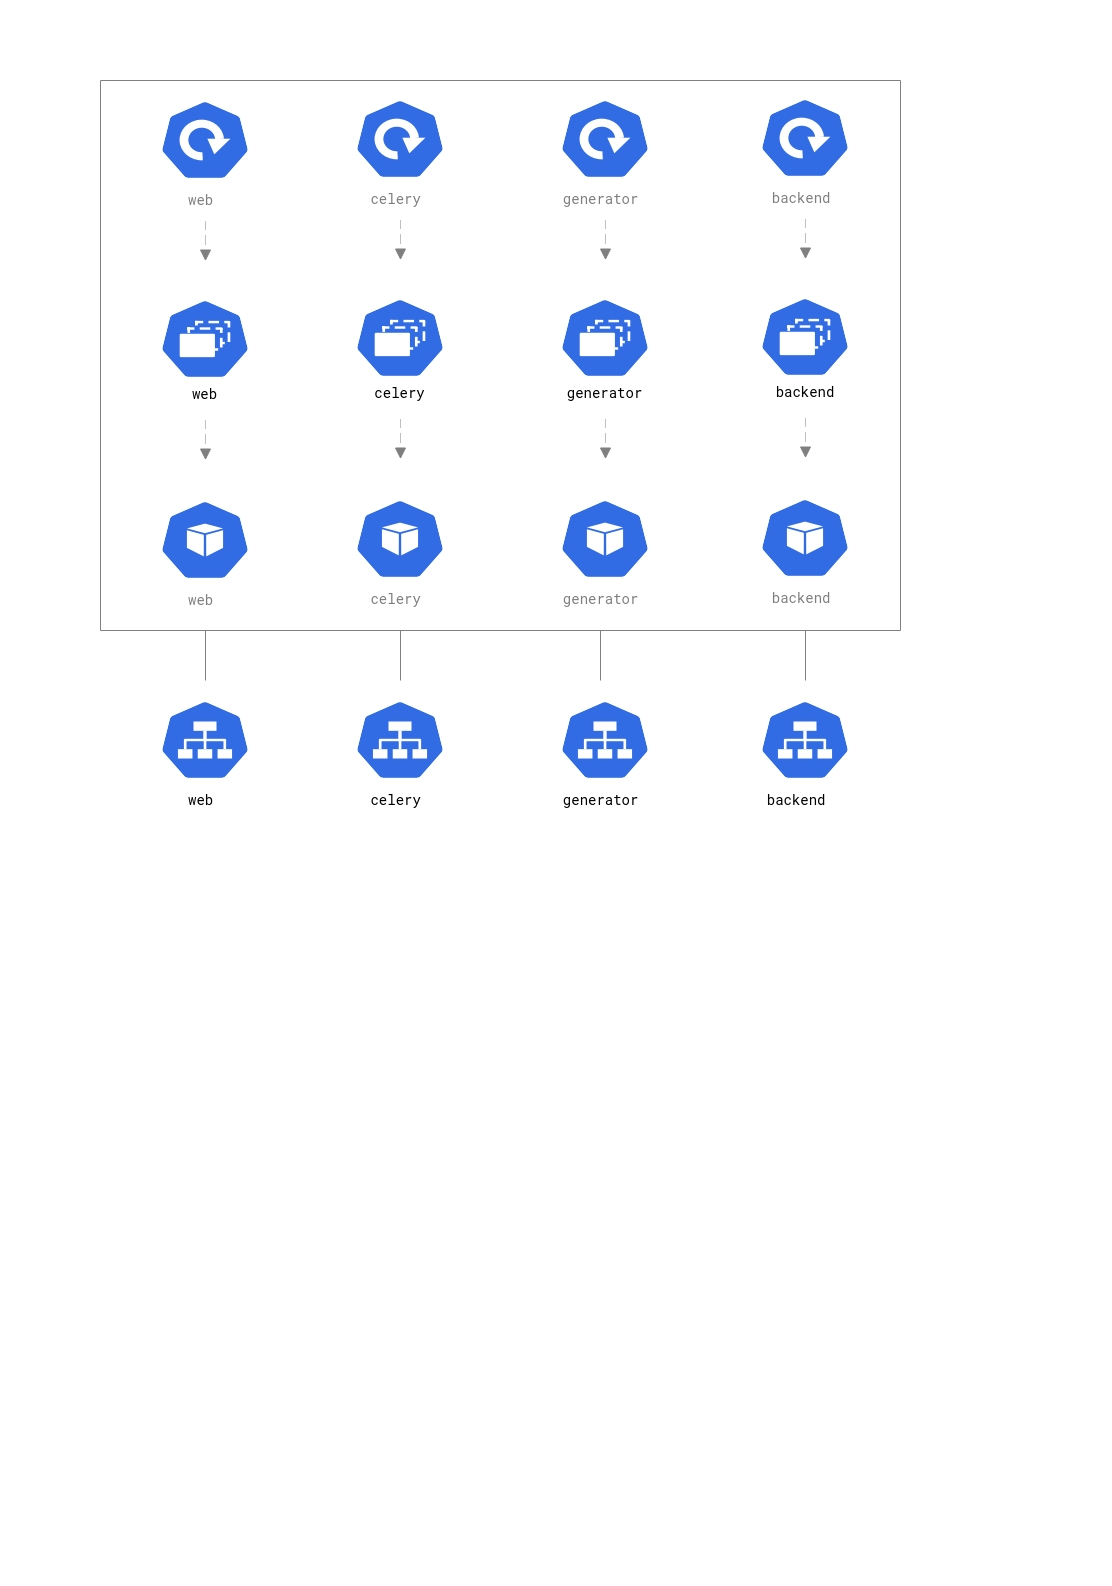
\includegraphics[scale=0.5]{deployment-diagram}
\end{figure}

\subsubsection{Backend}

\subsubsection{Web}

\subsubsection{Generator}

\subsection{StatefulSets}

\subsubsection{Postgres chart}
\begin{figure}[H]
\centering
\caption{PostgreSQL Helm chart}
\hspace*{1cm}
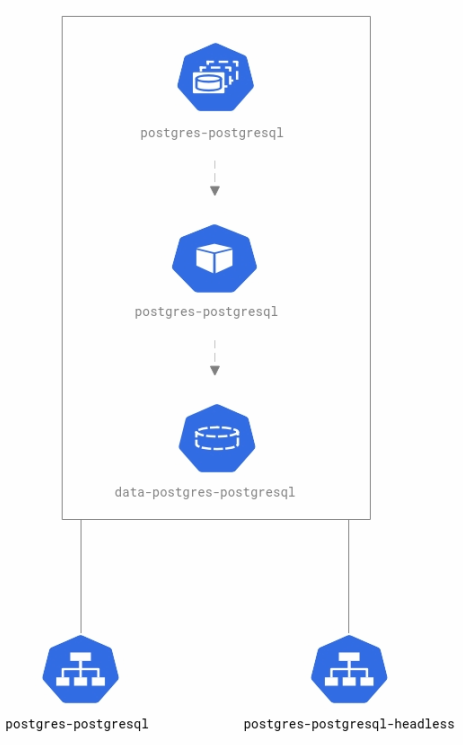
\includegraphics[scale=0.5]{postgres-diagram}
\end{figure}

\subsubsection{Redis chart}
\begin{figure}[H]
\centering
\caption{Redis Helm chart}
\hspace*{-3.4cm}
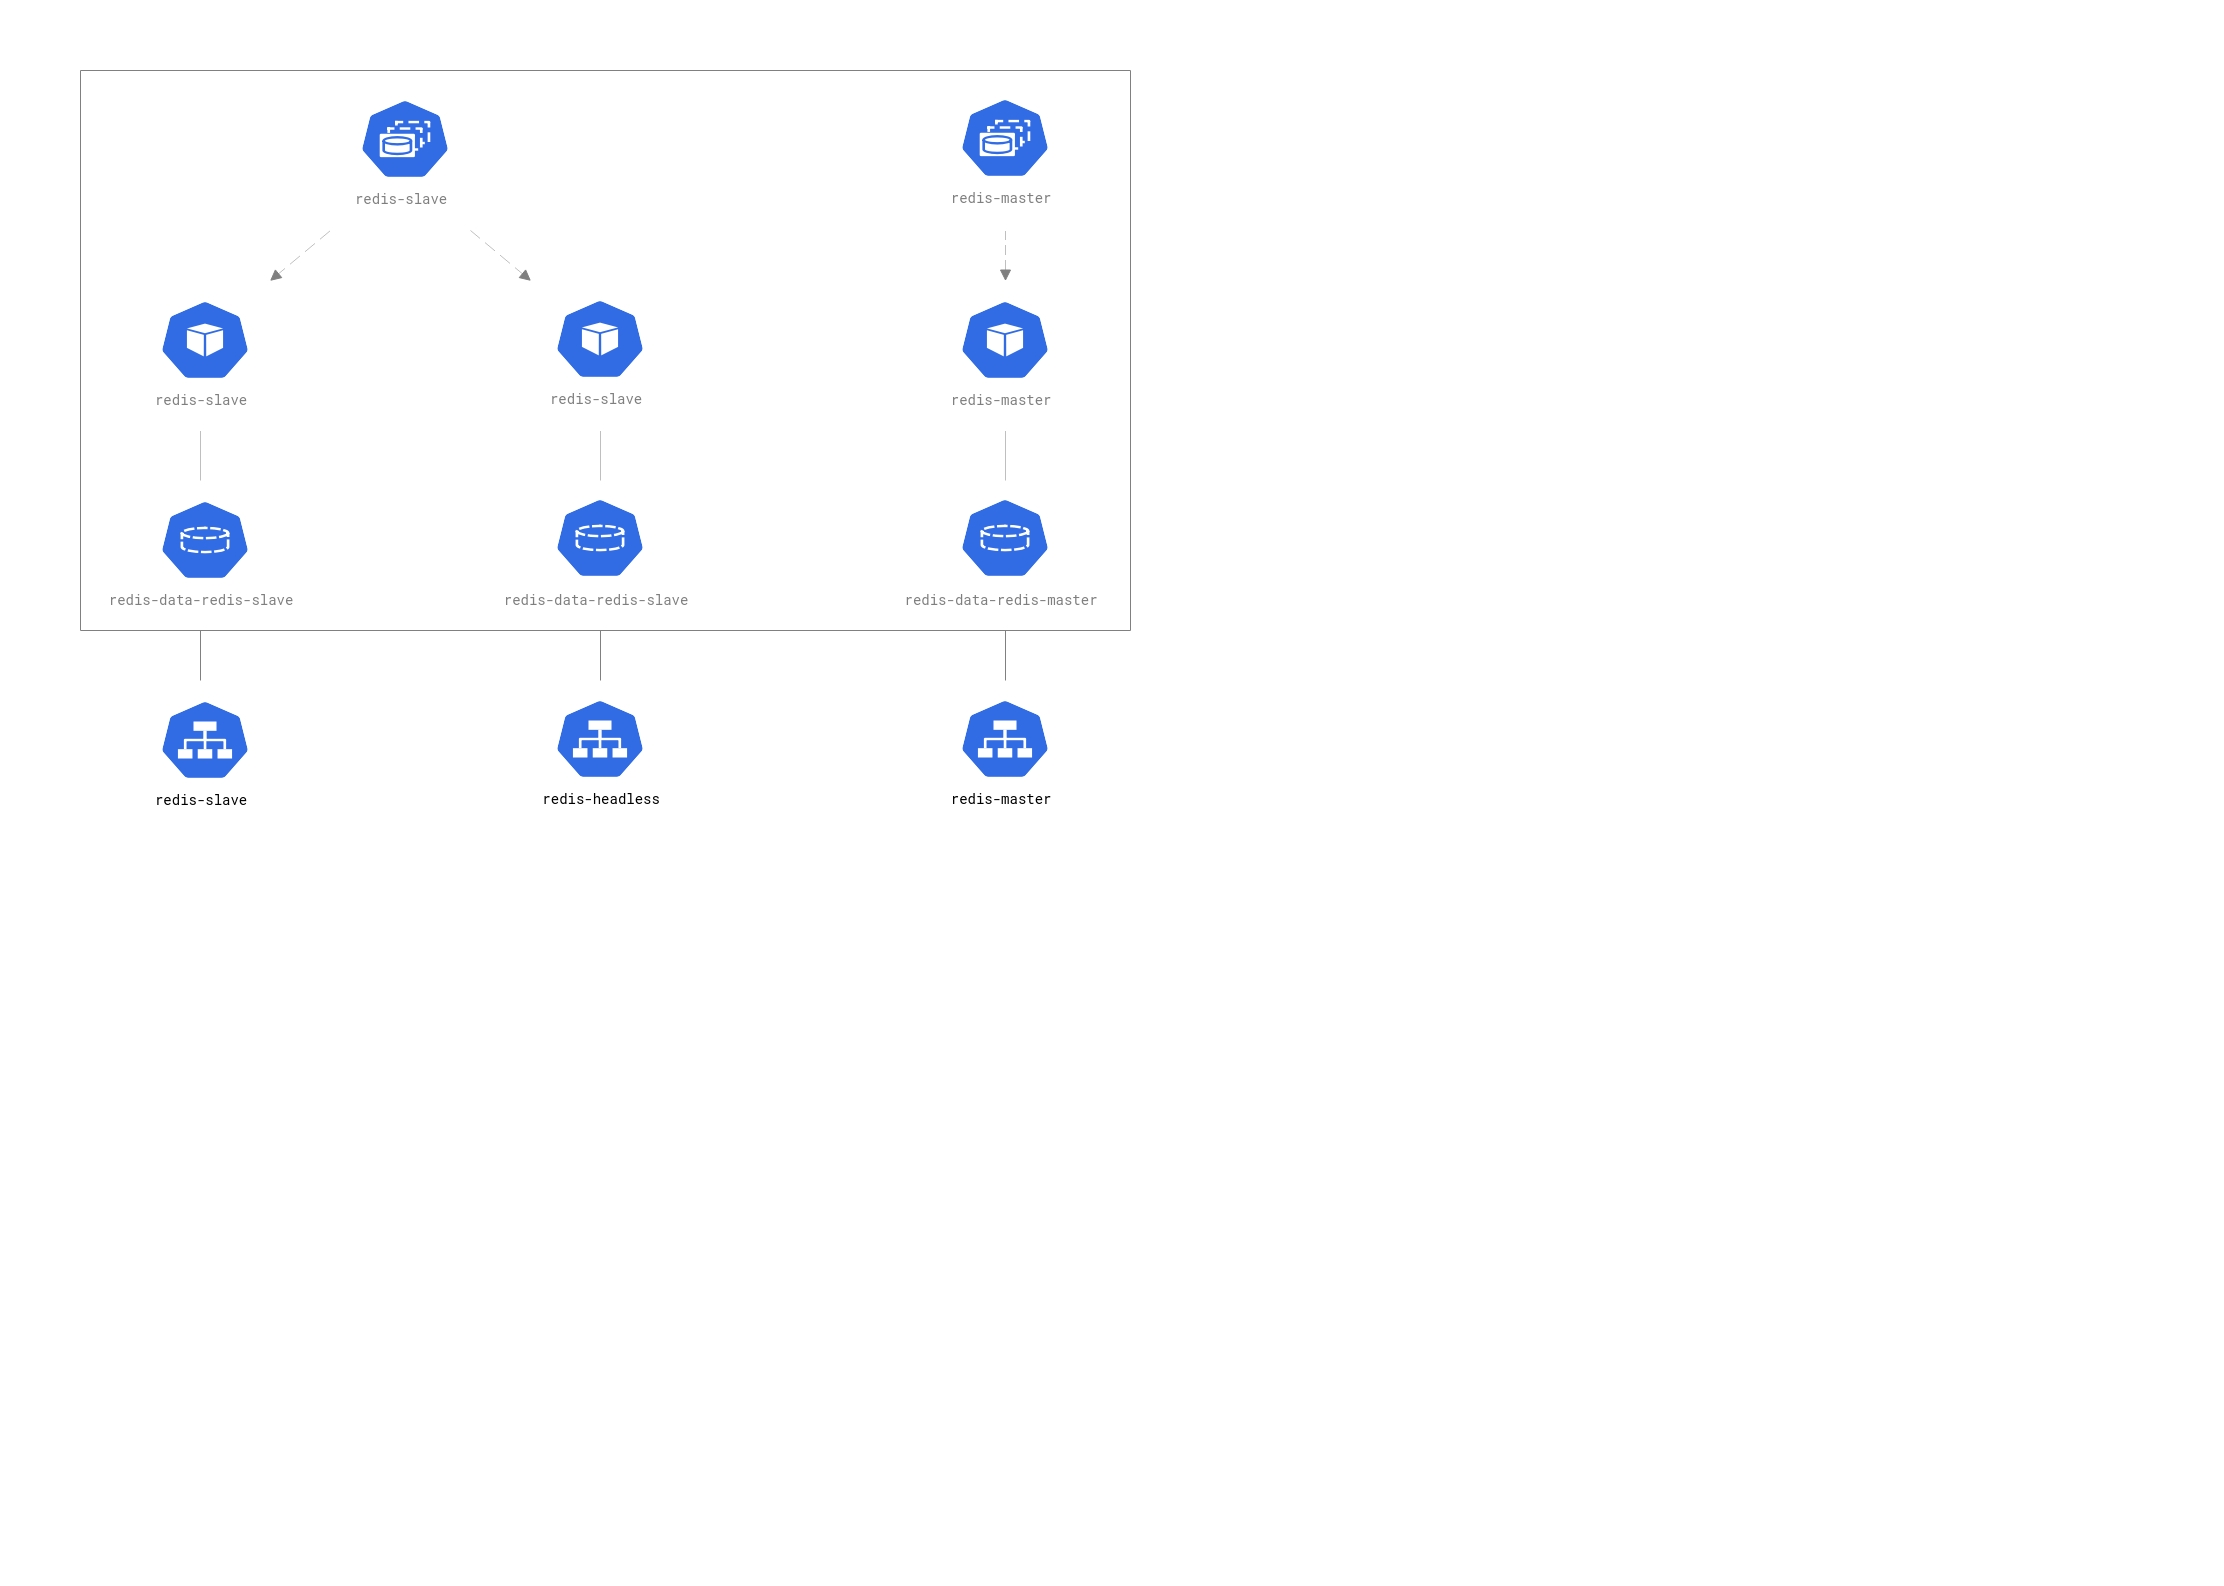
\includegraphics[scale=0.5]{redis-diagram}
\end{figure}

\subsection{Secrets}

\subsection{Configmaps}

\subsection{Ingress}

\subsubsection{Ingress chart}
\begin{figure}[H]
\centering
\caption{Ingress Helm chart}
\hspace*{1cm}
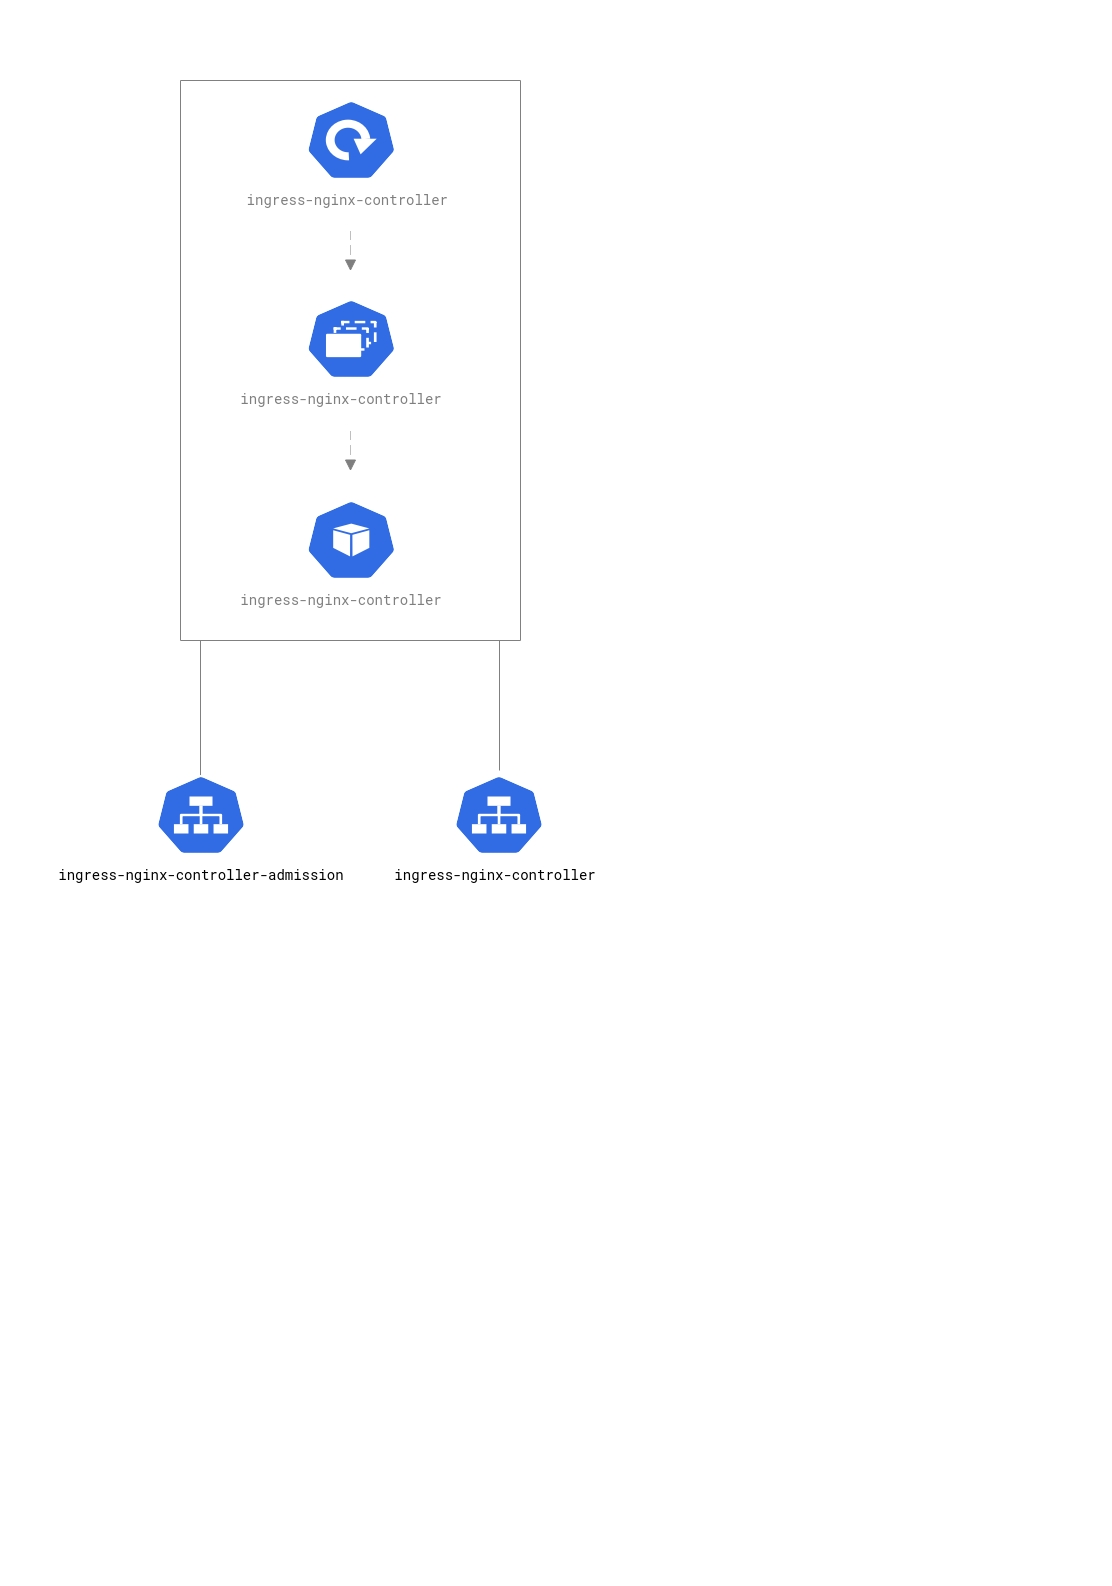
\includegraphics[scale=0.5]{ingress-diagram}
\end{figure}

\subsubsection{Ingress configuration}
\begin{figure}[H]
\centering
\caption{Ingress configuration of our cluster}
\hspace*{-3cm}
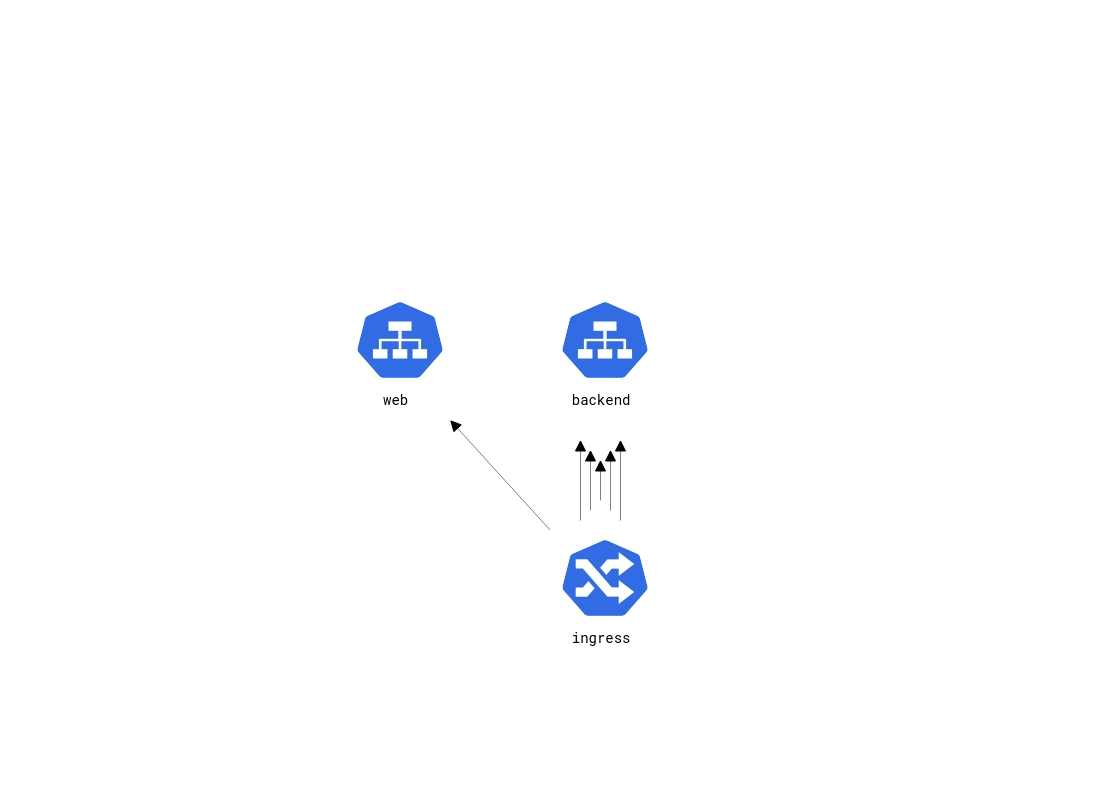
\includegraphics[scale=0.5]{exposed-services-diagram}
\end{figure}

\subsection{Scripts and Makefile}

\section{Gitlab CI/CD}

Finally, it is time to direct our attention to the implementation of a CI/CD pipeline by making use several of the tools from the large toolbox which is the Gitlab CI offering.
 
\subsection{Gitlab Container Registry}

\subsection{Gitlab Runners}

\subsection{Building pipelines}



\section{Future improvements}

In this final section of our thesis, we shall focus on potential improvements for the next iterations of the LearnShell Kubernetes cluster.





\setsecnumdepth{part}
\chapter{Conclusion}

In closing, let us walk through the goals set in this thesis. 
\newline
In the first chapter, we reviewed the current infrastructure architecture of LearnShell, and proposed possible improvements, the chief one being building a cluster for scaling and load-balancing. Then, we have gone over the theoretical concepts behind modern cluster platforms, and talked about some of the most used technologies in the field. Afterwards, we analysed and scrutinized the suitability of technologies that would help us create that cluster, and used our acquired knowledge to create a project that would create a cluster from a combination of configuration files and commands, allowing the user to choose between an on-premises cluster and a cloud-based one (while discussing the pros and cons of each). Finally, as our last task, we implemented a CI/CD pipeline for each project where it was deemed necessary, by using our newly-created cluster to deploy Gitlab Runners. Additionally, we provided diagrams as well as code snippets from our project in order to shed light on our cluster infrastructure. 
\newline
The code is available for students and staff on a repository in the Gitlab server of the Czech Technical University in Prague. Moreover, we have organised the containers into private registries on Gitlab, and built pipelines around them via Gitlab CI.
\newline
While we feel confident that the goals were completed, there is always room for improvement; in this current iteration, the cluster can be used in practice as a staging environment for development, but to be truly production-ready, some additional work would be required, although we believe that in this state, LearnShell is well-situated to migrate completely to a cluster infrastructure in the near future.



\bibliographystyle{iso690}
\bibliography{citations}


\setsecnumdepth{all}
\appendix

\chapter{Acronyms}
% \printglossaries
\begin{description}
	\item{GCP} Google Cloud Platform
	\item{GKE} Google Kubernetes Engine
	\item{CI} Continuous Integration
	\item{CD} Continuous Delivery
	\item{VM} Virtual Machine
	\item{K8S} Kubernetes
	
\end{description}


\chapter{Contents of enclosed CD}

%change appropriately

%\begin{figure}
%	\dirtree{%
%		.1 readme.txt\DTcomment{the file with CD contents description}.
%		.1 exe\DTcomment{the directory with executables}.
%		.1 src\DTcomment{the directory of source codes}.
%		.2 wbdcm\DTcomment{implementation sources}.
%		.2 thesis\DTcomment{the directory of \LaTeX{} source codes of the thesis}.
%		.1 text\DTcomment{the thesis text directory}.
%		.2 thesis.pdf\DTcomment{the thesis text in PDF format}.
%		.2 thesis.ps\DTcomment{the thesis text in PS format}.
%	}
%\end{figure}

\end{document}
